
\documentclass[english]{beamer}


% my default preamble

\usepackage{amsmath}
\usepackage{amssymb}
\usepackage{bm}
\usepackage{mathpazo}
% font setup
\usepackage[sfdefault,lf]{carlito}
\usefonttheme[onlymath]{serif}
\usepackage{xcolor}
\usepackage{tcolorbox}
\usepackage{hyperref}
\usepackage[round]{natbib}
\usepackage{adjustbox}
\usepackage{multicol}
\usepackage{array}
\usepackage{booktabs}
\usepackage{dcolumn}
\renewcommand{\arraystretch}{1.2} 

\newcounter{saveenumi}
\newcommand{\seti}{\setcounter{saveenumi}{\value{enumi}}}
\newcommand{\conti}{\setcounter{enumi}{\value{saveenumi}}}

% \newcommand{\newblock}{}

% \usepackage{enumitem}

% \usepackage{heuristica}
% \usepackage[heuristica,vvarbb,bigdelims]{newtxmath}
% \usepackage[T1]{fontenc}
% \renewcommand*\oldstylenums[1]{\textosf{#1}}

% \usepackage{lmodern}
% \usepackage[T1]{fontenc}

% \usepackage[bitstream-charter]{mathdesign}
% \usepackage[T1]{fontenc}

% \usepackage{cmbright}
% \usepackage[T1]{fontenc}
% \usetheme{Singapore}
% \setbeamertemplate{frametitle}[default][center]

% set some beamer templates
\setbeamertemplate{footline}[frame number] 
% \setbeamertemplate{caption}[numbered]
% \setbeamertemplate{footline}[frame number]{}
% \setbeamertemplate{navigation symbols}{}
% \setbeamertemplate{footline}{}
% different enumerates
\setbeamercolor{item projected}{bg=blue!80!black,fg=white}
\setbeamertemplate{enumerate items}[circle]
\setbeamertemplate{itemize items}[circle]
% define new commands
\newcommand{\red}[1]{{\color{red}{#1}}}
\newcommand{\blue}[1]{{\color{blue}{#1}}}
\newcommand{\bred}[1]{\textbf{\color{red}{#1}}}
\newcommand{\bblue}[1]{\textbf{\color{blue}{#1}}}

\newtcbox{\cyanbox}{on line, arc=1pt,left=1pt,right=1pt,top=1pt,bottom=1pt, colback=cyan!35!white, colframe=cyan!75!black,boxrule=1pt}
\newtcbox{\bluebox}{on line, arc=1pt,left=1pt,right=1pt,top=1pt,bottom=1pt, colback=blue!15!white, colframe=blue!80!black,boxrule=1pt}
\newtcbox{\redbox}{on line, arc=1pt,left=1pt,right=1pt,top=1pt,bottom=1pt, colback=red!5!white, colframe=red!75!black,boxrule=1pt}
\newtcbox{\greybox}{on line, arc=1pt,left=0.2pt,right=0.2pt,top=0.2pt,bottom=0.2pt, colback=black!5!white, colframe=white!75!black,boxrule=0.5pt}
\newcommand{\link}[2]{\greybox{\hyperlink{#1}{\texttt{#2}}}}
\newcommand{\slink}[2]{\greybox{\hyperlink{#1}{{\small\texttt{#2}}}}}

% \renewcommand<>{\item}{\beameroriginal\item\vspace{\stretch{.25}}}

% new variable linewidth environments
\newenvironment{smalli}
{ \begin{itemize}
    \setlength{\itemsep}{1pt}
    \setlength{\parskip}{1pt}
    \setlength{\parsep}{1pt}     }
{ \end{itemize}                  } 
\newenvironment{widei}
{ \begin{itemize}
    \setlength{\itemsep}{10pt}
    \setlength{\parskip}{10pt}
    \setlength{\parsep}{10pt}     }
{ \end{itemize}                  } 
\newenvironment{smalle}
{ \begin{enumerate}
    \setlength{\itemsep}{1pt}
    \setlength{\parskip}{1pt}
    \setlength{\parsep}{1pt}     }
{ \end{enumerate}                  } 
\newenvironment{widee}
{ \begin{enumerate}
    \setlength{\itemsep}{10pt}
    \setlength{\parskip}{10pt}
    \setlength{\parsep}{10pt}     }
{ \end{enumerate}                  } 
\newenvironment{mide}
{ \begin{enumerate}
    \setlength{\itemsep}{5pt}
    \setlength{\parskip}{5pt}
    \setlength{\parsep}{5pt}     }
{ \end{enumerate}                  } 
\newenvironment{midi}
{ \begin{itemize}
    \setlength{\itemsep}{5pt}
    \setlength{\parskip}{5pt}
    \setlength{\parsep}{5pt}     }
{ \end{itemize}                  } 

\begin{document}


\title{Estimation of DP Models}

\subtitle{ScPo CompEcon}


\frame{\titlepage} 

\frame{\frametitle{Table of contents}\tableofcontents} 

\section{Rust Bus Replacement}

\begin{frame}
\tableofcontents[currentsection] 
\end{frame}





\begin{frame}{Estimation of Dynamic Programming Models}
\begin{midi}
\item Now that we know how to solve them, how do we estimate DP models?
\item Examples
\begin{itemize}
\item \cite{rustbus}
\item \cite{BLP}
\end{itemize}
\item There are many different methods. We will introduce just a few. Look at the survey \cite{Aguirre} for more details.
\end{midi}
\end{frame}

\begin{frame}{\cite{rustbus}}
\begin{itemize}
\item Each Bus comes in once a month for repair
\begin{itemize}
\item Harold Zurcher decides after observing mileage $x_t$ since last engine replacment \bred{and} some other unobserved variable $\varepsilon$ whether to replace or not:
\begin{equation*}
u(x+t,d_t,\red{\theta^c},\red{RC}) = \begin{cases}-c(x_t,\red{\theta^c}) & \text{if }d_t=0 \\ 
                                                  -(\red{RC} + c(0,\red{\theta^c}) & \text{if }d_t=1
  \end{cases}
\end{equation*}

\item He solves the DP
\begin{equation*}
V_\red{\theta}(x_t) = \sup_{d_t} \mathbb{E}\left\{ \sum_{j=t}^\infty \beta^{j-t} u(x_j,d_j,\red{\theta}) + \varepsilon_t(d_t) |x_t \right\}
\end{equation*}
\end{itemize}
\item Parameters to be estimated: $\red{\theta} = \red{(\theta^c,RC,\theta^p)}$
\item This formulation results after making a set of simplifying assumptions.
\end{itemize}
\end{frame}


\begin{frame}{\cite{rustbus}}
\begin{midi}
\item To simplify, the odometer progress is assumed to be a random process.
\item that is, $x_t$ evolves stochastically.
\item The assumption is that $x_{t+1}\in\{s,s+1,s+2,s+3\}$ where $s$ is the state of $x_t$, i.e. the bin it lies in. 
\end{midi}

\end{frame}
	
\begin{frame}{Model and Data}
\begin{midi}
\item Data: a time series $\{x_t,d_t \}_{t=1}^T$
\item Likelihood function is
\begin{equation*}
\mathcal{L}(\red{\theta}) = \Pi_{t=2}^T P(d_t|x_t,\red{\theta^c},\red{RC})p(x_t|x_{t-1},d_{t-1},\red{\theta^p})
\end{equation*}
where the conditional choice probabilities are given by
\begin{equation*}
P(d_t|x_t,\red{\theta^c},\red{RC}) = \frac{\exp[u(x,d,\red{\theta^c},\red{RC}) + \beta\blue{EV}_\red{\theta}(x,d)]}{\sum_{d'\in\{0,1\}}\exp[u(x,d',\red{\theta^c},\red{RC}) + \beta\blue{EV}_\red{\theta}(x',d')]}
\end{equation*}
and, importantly, $\blue{EV}$ is the solution to

\begin{align*}
\blue{EV}_\red{\theta}(x,d) =& T_\red{\theta}(\blue{EV}_\red{\theta})(x,d) \\
                       \equiv&\int_{x'=0}^\infty \log \left( \sum_{d'\in{0,1}}\exp[u(x,d',\red{\theta^c},\red{RC}) + \beta\blue{EV}_\red{\theta}(x',d')] \right)
\end{align*}
\end{midi}
\end{frame}


\begin{frame}{Nested Fixed Point Algorithm (NXFP)}
\begin{widee}
\item \bred{Outer Loop}: Solve the Likelihood function
\begin{equation*}
\max_{\red{\theta}>0} \mathcal{L}(\red{\theta}) = \Pi_{t=2}^T P(d_t|x_t,\red{\theta^c},\red{RC})p(x_t|x_{t-1},d_{t-1},\red{\theta^p})
\end{equation*}
\item \bblue{Inner Loop}: Compute Expected value function $\blue{EV}_\red{\theta}$ for a given guess $\red{\theta}$
\begin{equation*}
\blue{EV}_\red{\theta} = T_\red{\theta}(\blue{EV}_\red{\theta})(x,d)
\end{equation*}
\end{widee}
\end{frame}

\begin{frame}{Potential Issues with NXFP}
\begin{midi}
\item We need a stopping rule for the likelihood function.
\item We need one for the inner loop as well.
\item Errors will propagate from the inner loop to the outer loop.
\item Given that the search direction on $\mathcal{L}(\red{\theta})$ depends on it's gradient, errors will matter a lot.
\item the tolerance on the inner loop needs to be \bred{tight}, like $1.0e^{-13}$
\end{midi}
\end{frame}




\begin{frame}{MPEC}{Mathematical Programming with Equality constraints}

\begin{midi}
\item We can turn the problem around. 
\item Instead of asking \emph{Whats the \blue{EV} compatible with my guess $\red{\theta}$?}, we could directly attack the likelihood: 
\item Maximize $\mathcal{L}(\red{\theta})$ \bred{subject to} the constraint, that behavior is \bblue{optimal} according to the model.
\item in other words, augment the likelihood:
\end{midi}

\begin{align*}
\mathcal{L}(\red{\theta},\blue{EV};X) &= \Pi_{t=2}^T P(d_t|x_t,\red{\theta^c},\red{RC})p(x_t|x_{t-1},d_{t-1},\red{\theta^p}) \\
P(d_t|x_t,\red{\theta^c},\red{RC}) &= \frac{\exp[u(x,d,\red{\theta^c},\red{RC}) + \beta\blue{EV}(x,d)]}{\sum_{d'\in\{0,1\}}\exp[u(x,d',\red{\theta^c},\red{RC}) + \beta\blue{EV}(x',d')]}
\end{align*}

\end{frame}

\begin{frame}{Different Optimization problems}
\bred{NXFP} solves the unconstrained optimization problem:
\begin{equation*}
\max_{\red{\theta}} \mathcal{L}(\red{\theta},\blue{EV}_\red{\theta})
\end{equation*}
\bblue{MPEC} solves the constrained optimization problem:
\begin{align*}
\max_{\red{\theta},\blue{EV}} & \mathcal{L}(\red{\theta},\blue{EV};X) \\
\text{subject to} & \blue{EV} = T(\blue{EV},\red{\theta})
\end{align*}
\end{frame}

\begin{frame}{\cite{juddsu}}

\begin{midi}
\item \cite{juddsu} perform MPEC on the bus model.
\item the key difference to note is that $\blue{EV}$ now becomes a choice variable.
\item In fact, the optimizer will be fed a vector
\begin{equation*}
x = [RC,\theta^c,\mathbf{EV}]
\end{equation*}
where $\mathbf{EV}$ is an approximation to $\blue{EV}$. In \cite{juddsu}, this is just going to be 
\begin{equation*}
\mathbf{EV} \equiv [EV(x_1),EV(x_2),\dots,EV(x_n)]
\end{equation*}
i.e. the approximation needs to hold pointwise.
\end{midi}
\end{frame}

\begin{frame}{\cite{juddsu}}
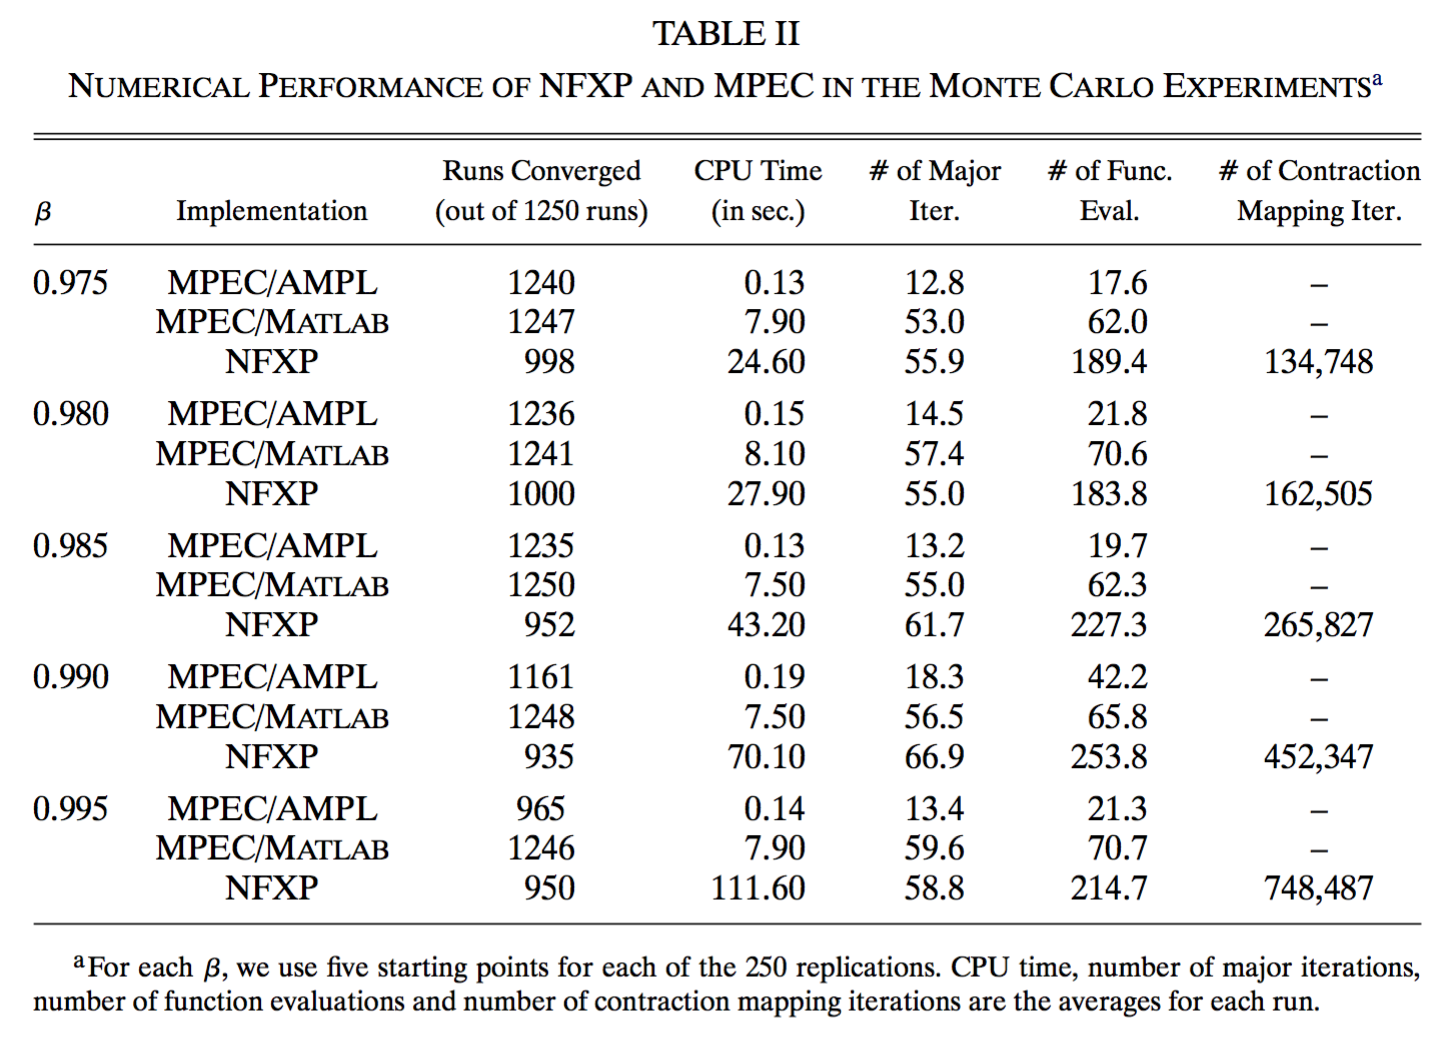
\includegraphics[width=11cm]{su-2.png}

\end{frame}

\begin{frame}{Performance}
\begin{midi}
\item In \emph{general}, NXFP is a computationally expensive operation.
\begin{itemize}
\item you have to solve a DP for many many many times in order to find your $\red{\theta}$.
\end{itemize}
\item However, there is much to qualify about this statement. The \bred{details} matter here.
\item For example, \cite{juddsu} are very critical about NXFP in the Bus Model. They compare it to the performance of \bblue{MPEC}.
\item But \citet{iskhakov2016comment} redo the exercise with Rust's original method to solve $\blue{EV}$ and show that NXFP is still a very strong contender in this example.
\end{midi}
\end{frame}


\section{Berry, Levinsohn and Pakes (BLP) as MPEC}

\begin{frame}
\tableofcontents[currentsection] 
\end{frame}
	
\begin{frame}{BLP after \cite{dube2012improving}}
\begin{midi}
\item \cite{BLP} is a model for automobile sales.
\item It has become a very widely applied model and estimation technique, short: \bred{BLP}.
\item The original paper performs demand estimation with a large number of differentiated products:
\begin{itemize}
\item characteristics approach
\item useful when only aggregate data are available
\item allows for flexible substitition patterns
\item controls for price endogeneity
\end{itemize}
\item The computational algorithm derives moment conditions from a non-linear model
\item The method is also known as \bblue{Random Coefficients Logit Demand} 
\end{midi}
\end{frame}

\begin{frame}{Random Coefficients Logit Demand}
\begin{midi}
\item The Utility of $i$ from purchasing product $j$ in market $t$ is
\begin{equation}
u_{ijt} = \red{\beta_i^0} + x_{jt}\red{\beta_i^x} - \red{\beta_i^p} p_{jt} + \blue{\xi_{jt}} + \varepsilon_{ijt} \label{eq:demand}
\end{equation}
\item with product characteristics $x_{jt},p_{jt},\blue{\xi_{jt}}$
\begin{itemize}
\item $x_{jt},p_{jt}$: ovserved with $cov(p_{jt},\blue{\xi_{jt}})\neq 0$
\item $\blue{\xi_{jt}}$: unovserved to econometrician.
\end{itemize}
\item $\red{\beta_i} \equiv [\red{\beta_i^0},\red{\beta_i^x},\red{\beta_i^p}]$: random coefficients or individual specific tastes to be estimated.
\begin{itemize}
\item We posit a distribution: $\red{\beta_i} \sim F_\beta(\beta,\red{\theta})$
\item \redbox{Goal of BLP}: estimate $\red{\theta}$ in the above parametric distribution.
\item errors are assumed type 1 EV
\item Consumer picks product $j$ if $u_{ijt}\geq u_{ij't}$
\end{itemize}
\end{midi}
\end{frame}

\begin{frame}{The Model: Market Shares}
\begin{midi}
\item The model predicts \cyanbox{market shares}:
\begin{equation}
s_j(x_t,p_t,\blue{x_{it}};\red{\theta}) = \int_{\{\beta_i,\varepsilon_i | u_{ijt}\geq u_{ij't},\forall j'\neq j\}} dF_\beta(\beta,\red{\theta}) dF_\varepsilon(\varepsilon)
\end{equation}
\item with type 1 EV shocks $\varepsilon$, there is an analytical solution to one of those integrals:
\begin{equation}
s_j(x_t,p_t,\blue{x_{it}};\red{\theta})  = \int_\beta \frac{\exp(\beta^0 + x_{jt}\beta^x - \beta^p p_{jt} + \blue{\xi_{jt}})}{1+\sum_{k=1}^J \exp(\beta^0 + x_{kt}\beta^x - \beta^p p_{kt} + \blue{\xi_{kt}})} dF_\beta(\beta,\red{\theta})
\end{equation}
\end{midi}
\end{frame}

\begin{frame}{The Model: Market Shares}
They use numerical integration:
\begin{equation}
\hat{s}_j(x_t,p_t,\blue{x_{it}};\red{\theta})  = \frac{1}{ns} \sum_{r=1}^{ns} \frac{\exp(\beta^{0r} + x_{jt}\beta^{xr} - \beta^{pr} p_{jt} + \blue{\xi_{jt}})}{1+\sum_{k=1}^J \exp(\beta^{0r} + x_{kt}\beta^{xr} - \beta^{pr} p_{kt} + \blue{\xi_{kt}})} dF_\beta(\beta,\red{\theta})
\end{equation}
to arrive at the market share (moment) conditions:
\begin{equation}
\hat{s}_j(x_t,p_t,\blue{\xi_{it}};\red{\theta}) = S_{jt},\forall j \in J,t\in T  \label{eq:shares}
\end{equation}
where $S_{jt}$ is data.
\end{frame}

\begin{frame}{GMM Estimator}
\begin{midi}
\item If firms can observe demand shocks $\blue{\xi_t}$, they will set prices accordingly.
\item There will be correlation between $p_t$ and $\blue{\xi_t}$ $\Rightarrow$ Endogeneity Bias!
\item BLP solve endogeneity of prices with a vector $z_{jt}$ of IVs, which are \bred{excluded} from the demand equation \eqref{eq:demand}
\item they propose a moment condition $E[\blue{\xi_{jt}}|z_{jt},x_{jt}] = 0 $
\item $z_{jt}$: e.g. product-specific cost shifters, or $K$ non-price characteristics in $x_{j,t}$ (assumed mean independent of $\blue{\xi_t}$)
\item We often form $E[\xi_{jt} \cdot h(z_{jt},x_{jt})] = 0 $ for some known function $h$.
\end{midi}
\end{frame}

\begin{frame}{Getting moment equations}
\begin{midi}
\item To get the sample analog of $E[\blue{\xi_{jt}}|z_{jt},x_{jt}] = 0$, we need to find $\blue{\xi_{jt}}$ corresponding to $\red{\theta}$
\item System \eqref{eq:shares} defines a mapping $\blue{\xi_{jt}}$ and $S_t$
\item Berry proved that $s$ has an inverse, hence any observed $S_t$ can be explained by a \bblue{unique} $\blue{\xi_{jt}}(\red{\theta}) = s^{-1}(S_t,\red{\theta})$
\item Sample analog of $E[\blue{\xi_{jt}}|z_{jt},x_{jt}] = 0$ is thus
\begin{equation*}
g(\red{\theta}) = \frac{1}{TJ}\sum_{t,j} \blue{\xi_{jt}}(\red{\theta})' z_{jt}
\end{equation*}
\end{midi}
\end{frame}

\begin{frame}{GMM Estimator}
\begin{widei}
\item Data are $\{(x_{jt},p_{jt},S_{jt},z_{jt})_{j\in J,t\in T}\}$
\item We want to minimize the GMM objective
\begin{equation*}
Q(\red{\theta}) = g(\red{\theta})' W g(\red{\theta})
\end{equation*}
\item There is no analytic form for $\blue{\xi_{jt}}(\red{\theta})$, see previous slide
\end{widei}
\end{frame}

\begin{frame}{\cite{BLP} Estimation Algorithm - NFXP}
\begin{midi}
\item \bred{Outer} Loop: $\min_{\red{\theta}} g(\red{\theta})' W g(\red{\theta})$
\begin{enumerate}
\item Guess vector $\red{\theta}$ to get $g(\red{\theta}) = \frac{1}{TJ}\sum_t \sum_j\blue{\xi_{jt}}(\red{\theta})' z_{jt}$
\item Stop whenever $|| \nabla_\theta(g(\red{\theta})' W g(\red{\theta})) || \leq \red{\epsilon_\text{out}}$
\end{enumerate}
\pause
\item \bblue{Inner} loop: compute $\blue{\xi_{jt}}(\red{\theta})$ given $\red{\theta}$
\begin{enumerate}
\item Solve system $s_j(x_t,p_t,\blue{x_{it}};\red{\theta}) = S_{\cdot t}$ by \bblue{Berry} constraction:
\begin{equation*}
\xi_t^{h+1} = \xi_t^{h} + \log S_t - \log s_j(x_t,p_t,\blue{\xi_{t}^h};\red{\theta})
\end{equation*}
\item Stop whenever $|| \xi_{\cdot t}^{h+1} - \xi_{\cdot t}^{h}  || \leq \red{\epsilon_\text{in}}$
\item Call resulting demand shock $\blue{\xi_{jt}}(\red{\theta},\red{\epsilon_\text{in}})$
\end{enumerate}
\item Clearly, need to choose \bred{both stopping rules} for inner and outer loop.
\end{midi}
\end{frame}

\begin{frame}{\cite{knittel2014estimation}}

\begin{midi}
\item They perform an extensive investigation into BLP on two widely used datasets: cars and cereals.
\item They use 10 free solvers and 50 starting points for each.
\item Find: convergence occurs at several local extrema, saddles, and in regions where the FOC is not satisfied.
\item Resulting parameter estimates of economic variables (market shares, price elasticiteis) exhibit \bred{huge} variation depending on solver/starting point.
\item All in all, they found 400 local solutions.
\end{midi}
\end{frame}

\begin{frame}{\cite{dube2012improving}'s concerns}
\begin{mide}
\item Too much computation
\begin{itemize}
\item need to know $\xi(\theta)$ only at true $\theta$.
\item NFXP solves for $\xi(\theta)$ at each stage.
\end{itemize}
\item Stopping criteria
\begin{itemize}
\item inner loop can be slow to converge
\item it's tempting to loosen $\red{\epsilon_\text{in}}$ (often see $\red{\epsilon_\text{in}}=1e^{-6}$ or higher!)
\item outer loop may not converge with loose inner criterion
\end{itemize}
\item Inner loop error propagates to outer loop.
\end{mide}
\end{frame}

\begin{frame}{Errors from loose stopping}
\begin{align*}	
\theta^* = & \arg \max_{\theta} Q(\xi(\theta,0)) \\
\hat{\theta} = & \arg \max_{\theta} Q(\xi(\theta,\red{\epsilon_\text{in}})) 
\end{align*}	
\begin{midi}
\item \cite{dube2012improving} derive bounds on the order of estimatin error as a function of $\red{\epsilon_\text{in}}$
\item Consider \cite{knittel2014estimation} for numerical experiments.
\end{midi}
\end{frame}

\begin{frame}{BLP as an MPEC}
\begin{midi}
\item \cite{dube2012improving} cast this as an MPEC:
\begin{align*}
\min_{\red{\theta},\blue{\xi}} & \blue{\xi}^T ZWZ^T\blue{\xi} \\
\text{subject to } & s(\blue{\xi},\red{\theta}) = S
\end{align*}
\item Advantages:
\begin{enumerate}
\item No need to set up 2 tolerances
\item no inner errors propagated
\item easy to code in AMPL
\item fewer iterations, given that AMPL provides analytic gradients/hessian
\end{enumerate}
\end{midi}
\end{frame}

\begin{frame}{Exploring Sparsity in BLP}
\begin{midi}
\item The way this is formulated now, the Hessian of objective is dense. :-(
\item They add an additional variable $\blue{r}$ and associated constraint $Z^T \blue{\xi}=\blue{r}$
\begin{align*}
\min_{\red{\theta},\blue{\xi},\blue{r}} & \blue{r}^T W \blue{r} \\
\text{subject to } & s(\blue{\xi},\red{\theta}) = S \\
\text{ and       } & Z^T \blue{\xi}=\blue{r}
\end{align*}
\item advantages: 
\begin{enumerate}
\item Hessian of objective function is now sparse
\item Very big saving in memory requirements.
\end{enumerate}
\end{midi}
\end{frame}

\begin{frame}{Convergence and Loose vs Tight}
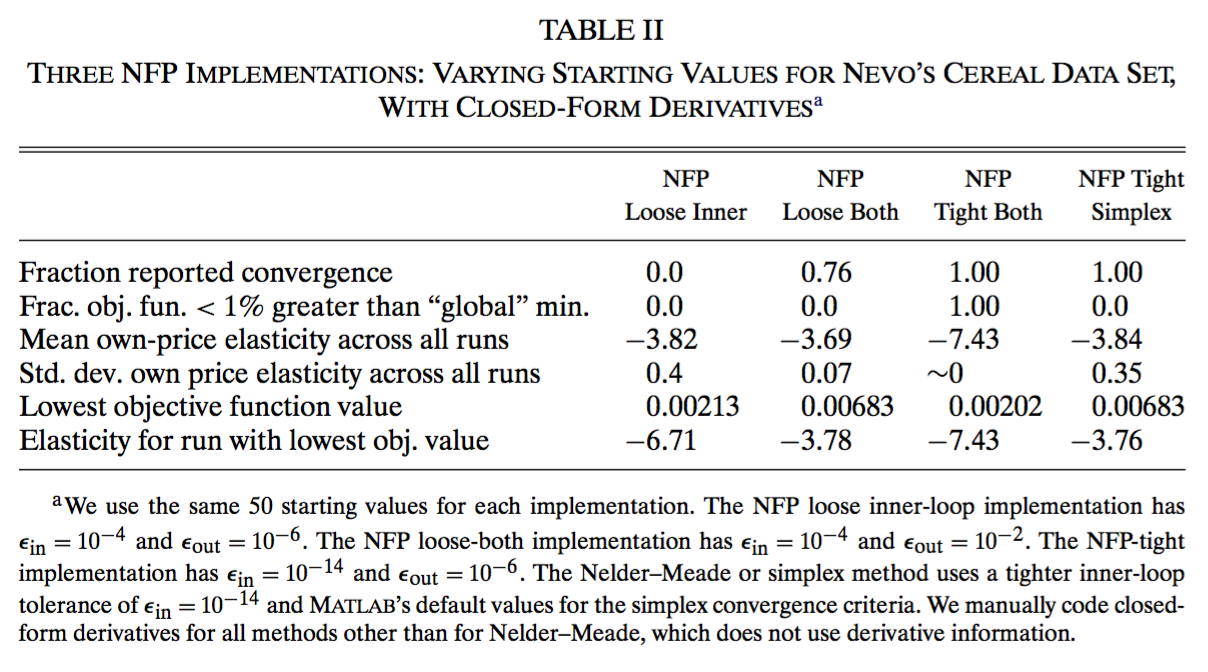
\includegraphics[width=10cm]{dube-2.png}

\end{frame}

\begin{frame}{Speed}
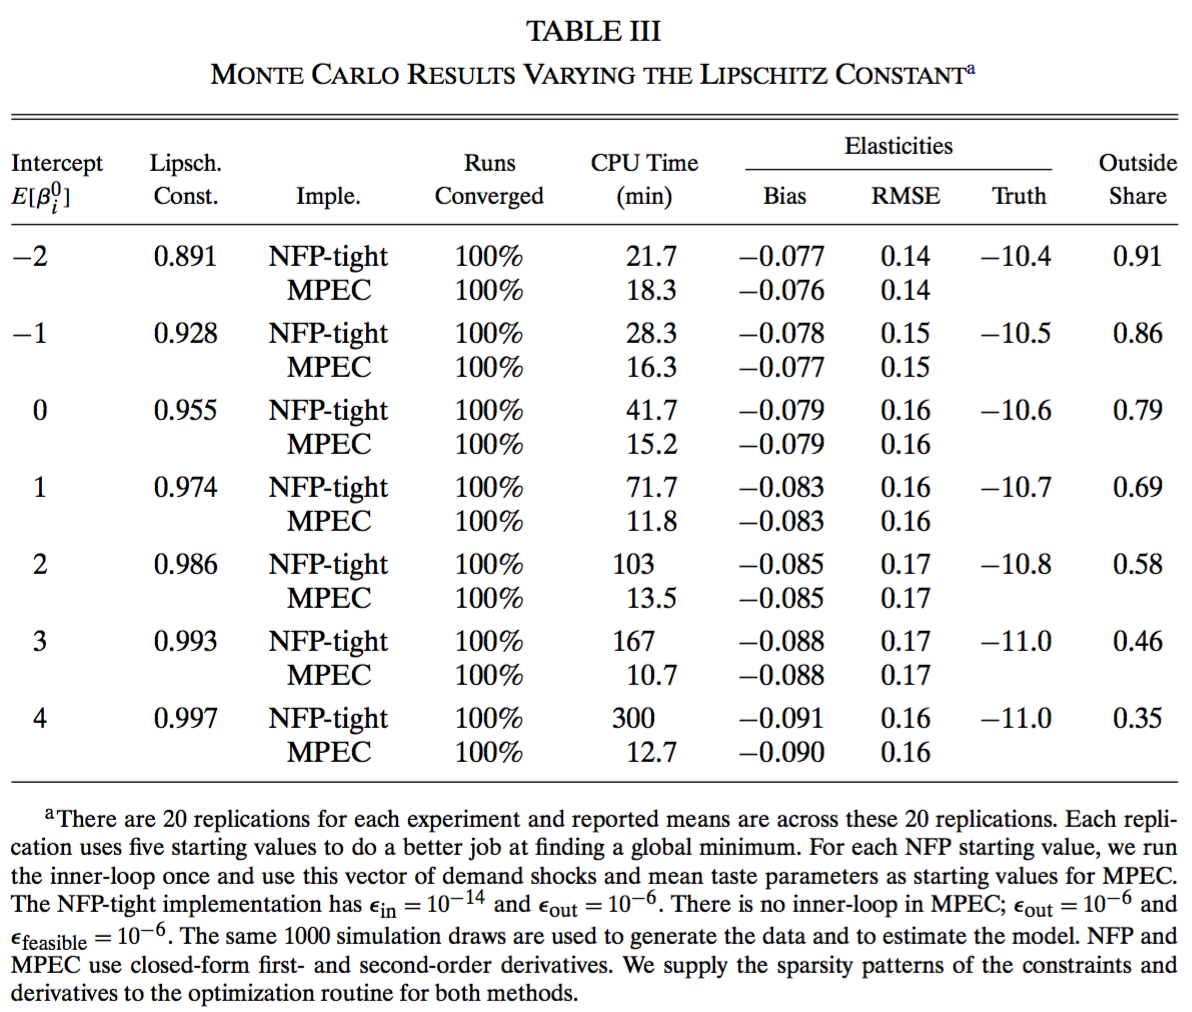
\includegraphics[width=10cm]{dube-3.png}

\end{frame}

\begin{frame}[allowframebreaks]{References}

        % \frametitle{References}
		\bibliographystyle{unsrtnat}
		\bibliography{../../references/references.bib}
\end{frame}


\end{document}
